\section{Results and Discussion}

\subsection{What conditions promote the evolution of phenotypic plasticity?}

Ghalambor \textit{et al.} identified four environmentally-dependent requirements for the evolution of phenotypic plasticity
\citep{ghalambor_behavior_2010}. 
Our experimental design conforms to these conditions, enabling us to test their validity and relative importance. 
The oscillation between ENV-NAND and ENV-NOT provides temporal variation. 
The IO-Sense instruction reliably indicates the current environment. 
The two environments favor opposing phenotypic traits, and the only way for an individual organism to achieve a high fitness in both environments is to alter its phenotypic expression. 
Given the existing theoretical and empirical support for these conditions, we expected to see the evolution of phenotypic plasticity in each of our experimental treatments. 
However, we were unsure of the impact of altering environmental factors such as mutation rate and environment fluctuation rate. 

% Report plasticity results. 
At the end of the experiment, we extracted the dominant (most abundant) genotype from the population of each replicate.
We tested these genotypes in both ENV-NAND and ENV-NOT and recorded each genotype's expressed phenotype across both environments. 
In Table \ref{chapter:origins-of-plasticity:table:evolutionary-outcomes}, we report the number of replicates in which the dominant genotype at the end of the experiment was plastic and the number of replicates in which the dominant genotype was optimally plastic. 
Note that for these results we only evaluated the most abundant genotype at the end of the experiment. 
An ancestor of the evaluated genotype may have been plastic, but if that plasticity was not maintained in the lineage, we did not count it in Table \ref{chapter:origins-of-plasticity:table:evolutionary-outcomes}. 

% More specifically report results
As expected, the capacity for phenotypic plasticity evolved in each experimental treatment; in 31 of the 50 baseline treatment replicates, phenotypic plasticity was present in the final dominant organism. 
None of the final dominant genotypes from the control replicates were phenotypically plastic. 
In all control replicates, the dominant genotype performed both the NAND and NOT tasks unconditionally. 
Our results are consistent with existing theoretical and empirical work, supporting the validity of the conditions likely to facilitate the evolution of phenotypic plasticity \citep{clune_investigating_2007,ghalambor_behavior_2010,hallsson_selection_2012,nolfi_phenotypic_1994}. 

\begin{table*}[t]
\renewcommand{\arraystretch}{1.5}
	\centering
    \small
    \begin{tabulary}{\textwidth}{| l | r | r | r | r | r |}
      \hline 
      \multicolumn{1}{| c |}{\centering \textbf{Treatment}} &
      \multicolumn{2}{ c |}{\centering \textbf{Plastic Replicates}} &
      \multicolumn{2}{ p{0.25\textwidth}|}{\centering \textbf{Unconditional Precedes Conditional}} & \multicolumn{1}{p{0.20\textwidth}|}{\centering \textbf{Sub-optimal Precedes Optimal}} \\
      \cline{2-5}
      & \multicolumn{1}{p{0.1\textwidth} |}{\centering Total} & \multicolumn{1}{p{0.1\textwidth} |}{\centering Optimal$^{*}$} & \multicolumn{1}{p{0.1\textwidth} |}{\centering NAND Task} & \multicolumn{1}{p{0.1\textwidth} |}{\centering NOT Task} & \\
      \hline 
      Baseline 						 & 31 (62\%) & 17 (34\%) & 31 (100\%)   & 28 (90.3\%) & 16 (94.1\%) \\
      \hline 
      Low Mutation Rate 			 & 38 (76\%) & 30  (60\%) & 34 (89.5\%) & 35 (92.1\%) & 30 (100\%) \\
      \hline 
      High Mutation Rate  			 & 25 (50\%) & 11  (22\%) & 25 (100\%)  & 24 (96\%)  & 10 (90.9\%) \\
      \hline 
      \parbox[t]{0.2\textwidth}{Short Environment Cycle Length} & 36 (72\%) & 18  (36\%) & 33 (91.7\%) & 28 (77.8\%) & 18 (100\%) \\
      \hline 
      \parbox[t]{0.2\textwidth}{Long Environment Cycle Length}  & 16 (32\%) & 10  (20\%) & 14 (87.5\%) & 16 (100\%)  & 9 (90\%) \\
      \hline 
      Control						 & 0 (0\%) & 0 (0\%) & \multicolumn{1}{c|}{--} & \multicolumn{1}{c|}{--} & \multicolumn{1}{c|}{--} \\
      \hline 
    \end{tabulary}
    \begin{tablenotes}
          \item[*] $^{*}$\small{Optimal is defined as the complete phenotype that only performs the rewarded task in each environment.}
    \end{tablenotes}
    \caption{\small 
    \textbf{A summary of evolutionary outcomes across all five experimental treatments and control.}
    Plastic Replicates indicates the number of replicates (out of 50 per treatments) in which the final dominant genotype was plastic at all (Total) and perfectly plastic (Optimal).  
    Unconditional Precedes Conditional indicates the number of times the NAND task and NOT task were expressed unconditionally before eventually evolving to be express conditionally (out of total plastic).  
    Finally, Sub-optimal Precedes Optimal indicates how many runs had an imperfect form of plasticity before eventually evolving to be optimally plastic (out of total optimally plastic).
    }
    \label{chapter:origins-of-plasticity:table:evolutionary-outcomes}
\end{table*}

\subsection{How do environmental factors impact the evolution of phenotypic plasticity?}

While our results show phenotypic plasticity can evolve under the conditions identified in \citep{ghalambor_behavior_2010}, how do mutation rate and fluctuation rate affect the evolution of phenotypic plasticity under these conditions? 
We found compelling results for both mutation rate and environmental cycle length. 

\subsubsection{Mutation Rate}

While only of borderline statistical significance ($p = 0.058$ using Fisher's Exact Test with Bonferroni corrections for multiple comparisons; all statistics were done in R version 3.2.2 \citep{r_core_team_2016}), our results trend such that populations at lower mutation rates appear more likely to evolve phenotypic plasticity than do populations at higher mutation rates. 
The most abundant genotypes exhibited some plasticity in 38/50 runs at a low mutation rate, 31/50 at the baseline mutation rate, and 25/50 and the high mutation rate.  
While higher mutation rates increase genetic variation from one generation to the next, most mutations that have phenotypic effects are deleterious \citep{sniegowski_evolution_2000}. 
Thus, at higher mutation rates, the elevated influx of deleterious mutations could increase the difficulty of maintaining the necessary genetic machinery for phenotypic plasticity.
Qualitative evidence for this effect can be seen in the time-sliced visualized lineages of final dominant, non-plastic genotypes from the high-mutation-rate treatment (Figure \ref{chapter:origins-of-plasticity:fig:high-mut-lineages}) where lineages traverse states of plasticity for some time before reverting back to states of non-plasticity\footnote{
For fully interactive visualizations of evolved lineages from all treatments, see \url{https://lalejini.com/evo-origins-of-phenotypic-plasticity-web/}
}.
Furthermore, more phenotypic shifts in general increase the probability of quickly finding an appropriate non-plastic phenotype after each environmental change.

\begin{figure*}[ht]
  \centering
  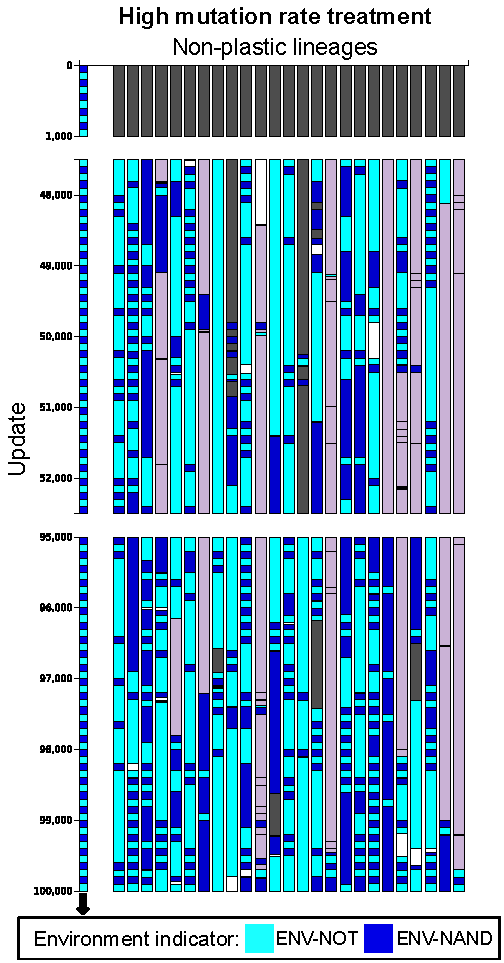
\includegraphics[height=0.5\textheight, keepaspectratio]{chapters/02-evolutionary-origins-of-plasticity/media/high-mutation-rate-non-plastic-lineages.pdf}
  \caption{\small 
  \textbf{Time-sliced visualization of lineages for non-plastic, dominant genotypes from the high-mutation-rate treatment.}
  Abbreviated color reference: 
  cyan represents unconditional NOT task performance, 
  dark blue represents unconditional NAND task performance, 
  and light purple represents sub-optimal forms of plasticity.  
  Refer to Figure \ref{chapter:origins-of-plasticity:fig:task-profiles} for a full legend of phenotype colors.}
  \label{chapter:origins-of-plasticity:fig:high-mut-lineages}
\end{figure*}



% Plastic lineages from the baseline treatment
\begin{figure*}[!ht]
  \centering
  \begin{minipage}[b]{\linewidth}
  \centering
  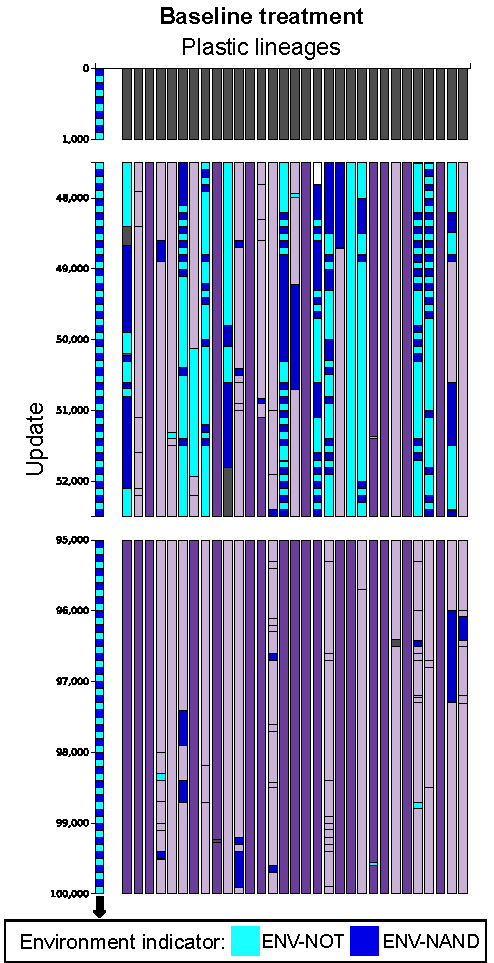
\includegraphics[height=0.5\textheight, keepaspectratio]{chapters/02-evolutionary-origins-of-plasticity/media/baseline-plastic-lineages.pdf}
  \caption{\small 
  Time-sliced lineage visualization of dominant, plastic genotypes from the baseline treatment. 
  Abbreviated color reference: 
  cyan represents unconditional NOT task performance, 
  dark blue represents unconditional NAND task performance, 
  light purple represents sub-optimal forms of plasticity, 
  and dark purple represents optimal plasticity.  
  Refer to Figure \ref{chapter:origins-of-plasticity:fig:task-profiles} for a full legend of phenotype colors.}
  \label{chapter:origins-of-plasticity:fig:baseline-lineages}
  \end{minipage}
\end{figure*}

\subsubsection{Environment Fluctuation Rate}

We found a significant difference ($p = 0.00028$ using Fisher's Exact Test with Bonferroni corrections for multiple comparisons) as we varied the cycle length for environmental switching.  
Specifically, in the long-environment-cycle-length, only 16/50 runs ended with a final dominant genotype that was phenotypically plastic, while the baseline and short-environment-cycle-length produced 31 and 36 plastic outcomes, respectively.

We expect that the short-environment-cycle-length treatment is biased toward the evolution of phenotypic plasticity because of the rapid environment fluctuations relative to other experimental treatments. 
Rapid fluctuations cause lineages to be less able to rely on mutational input for adaptation. 
In the long-environment-cycle-length treatment, environmental fluctuations may not occur rapidly enough to produce a sufficient selective pressure for phenotypic plasticity, allowing alternative adaptive strategies to evolve instead.

\subsection{What are the evolutionary stepping stones for phenotypic plasticity?}

In an attempt to identify patterns frequently encountered during the evolution of phenotypically plastic organisms, we extracted and analyzed the full lineages from our experiments. 
We tested each ancestor genotype in both ENV-NAND and ENV-NOT and classified their phenotype across both environments. 
In addition to a quantitative analysis, we also visualized the lineages of the dominant, plastic genotypes; see Figure \ref{chapter:origins-of-plasticity:fig:baseline-lineages} for the visualization of the baseline treatment. 
Using our visualizations and ancestor phenotype classifications, we addressed the following two questions: 
(1) Do the lineages of phenotypically plastic organisms first evolve to perform tasks unconditionally before evolving to perform them conditionally as a function of their current environment? 
And (2), do imperfect forms of phenotypic plasticity tend to precede optimal forms?

\subsubsection{Unconditional task performance precedes plasticity}

To explore whether or not unconditional task performance was an evolutionary stepping stone for conditional task performance (\textit{i.e.}, phenotypic plasticity), we determined whether a task was performed unconditionally prior to being performed conditionally by the ancestors of plastic genotypes. 
We analyzed both tasks (NAND and NOT) separately. These results are reported in Table \ref{chapter:origins-of-plasticity:table:evolutionary-outcomes}. 
% Answer to: unconditional before conditional?
Across all experimental treatments, non-plastic ancestors generally preceded plastic ancestors. 
In other words, unconditional task performance of the NAND and NOT tasks generally preceded the conditional performance of either task. 
Examples of this can be seen in time-sliced plastic lineages from the baseline treatment (Figure \ref{chapter:origins-of-plasticity:fig:baseline-lineages}) where many lineages maintain states of unconditional task expression prior to entering states of conditional task expression. 
These results suggest that, in fluctuating environments similar to those in our experiment, the evolutionary path to phenotypic plasticity usually traverses states of unconditional trait expression prior to entering states of conditional trait expression. 
This result should be unsurprising. 
In order to evolve a regulated function, the capacity for both the regulation and the function must exist. 
In our experiment, the function can be selected for without regulation; however, regulation of the function is unlikely to be selected for without the prior capacity for the function. 

\subsubsection{Sub-optimal plasticity precedes optimal plasticity}

To investigate sub-optimal phenotypic plasticity as an evolutionary stepping stone for optimal phenotypic plasticity in our experiment, we analyzed lineages of optimally plastic genotypes. 
Again, we consider only complete phenotypes that exclusively perform the rewarded task in each environment to be optimal. 
For each optimally plastic genotype's lineage, we determined whether or not the evolution of optimal plasticity was preceded by the evolution of sub-optimal phenotypic plasticity. 
The results of this analysis are reported in Table \ref{chapter:origins-of-plasticity:table:evolutionary-outcomes}.

% Answer to: sub-optimal before optimal?
Across all experimental treatments, the evolution of sub-optimal plasticity did, indeed, generally precede the evolution of optimal phenotypic plasticity.
Examples of sub-optimal plasticity preceding more optimal forms of plasticity can be seen in some of the time-sliced lineages from the baseline treatment visualized in Figure \ref{chapter:origins-of-plasticity:fig:baseline-lineages}. 
These results suggest that, in fluctuating environments similar to those in our experiment, sub-optimal forms of phenotypic plasticity tend to arise before the evolution of optimal forms of phenotypic plasticity. 

Unconditional trait expression tends to evolve first; then, sub-optimal forms of plasticity appear before optimal forms finally evolve.
While challenging to verify, we expect our results to be applicable to biological systems. 
The evolution of complex functions (\textit{e.g.}, optimal phenotypic plasticity) build on simpler, previously evolved functions (\textit{e.g.}, unregulated or sub-optimally regulated functions) \citep{lenski_evolutionary_2003}. 
These results, however, are particularly useful for applied evolutionary computation. 
If an evolved problem solution must respond dynamically to environmental variables, it is likely that the solution will need to be able to traverse through states of rigidity and sub-optimal plasticity prior to reaching a state of optimal plasticity. 
Thus, first evolving rigid solutions in fixed environments and then gradually starting to fluctuate more aspects of the environment over time could provide a scaffolding for the evolution of optimally plastic solutions.  

\subsection{Does plasticity still evolve when evolutionary stepping stones are disallowed?}

% Describe experiment
% - To investigate the importance of each of our observed stepping stones (unconditional trait expression and sub-optimal plasticity), we conducted a followup set of experiments.
We conducted a series of followup experiments to investigate the importance of unconditional trait expression and sub-optimal plasticity as evolutionary stepping stones.
We evolved 200 replicate populations under baseline treatment conditions (described in Section \ref{chapter:origins-of-plasticity:sec:methods:experimental-design}) and 200 replicate populations in each of three experimental conditions where we disallowed particular phenotypic profiles from evolving: (1) we disallowed phenotypes that expressed NAND and/or NOT unconditionally (\textit{i.e.}, task profiles 2, 3, and 4 from Figure \ref{chapter:origins-of-plasticity:fig:task-profiles}); (2) we disallowed sub-optimally plastic phenotypes (\textit{i.e.}, task profiles 5 through 8 and 10 through 16 from Figure \ref{chapter:origins-of-plasticity:fig:task-profiles}); and, (3) we disallowed phenotypes that exhibited unconditional trait expression \textit{or} phenotypes that were sub-optimally plastic (\textit{i.e.}, all task profiles except 1 and 9 from Figure \ref{chapter:origins-of-plasticity:fig:task-profiles}).
Note that in each of these experimental treatments, we always allowed phenotypes that expressed no tasks or were optimally plastic across both environments.
In treatments where particular phenotypes were disallowed, we tested all offspring in both ENV-NAND and ENV-NOT; if the phenotype of an organism's offspring was among the disallowed phenotypes, we prevented its birth.
As in our previous experiments, we counted the number of replicates of each treatment where the dominant genotype at the end of the experiment exhibited a plastic phenotype.
% @AML: should give each experimental treatment a name (e.g., no-unconditional-expression, no-sub-optimal-plasticity, and no-intermediate-phenotypes)

\begin{figure*}[!ht]
  \centering
  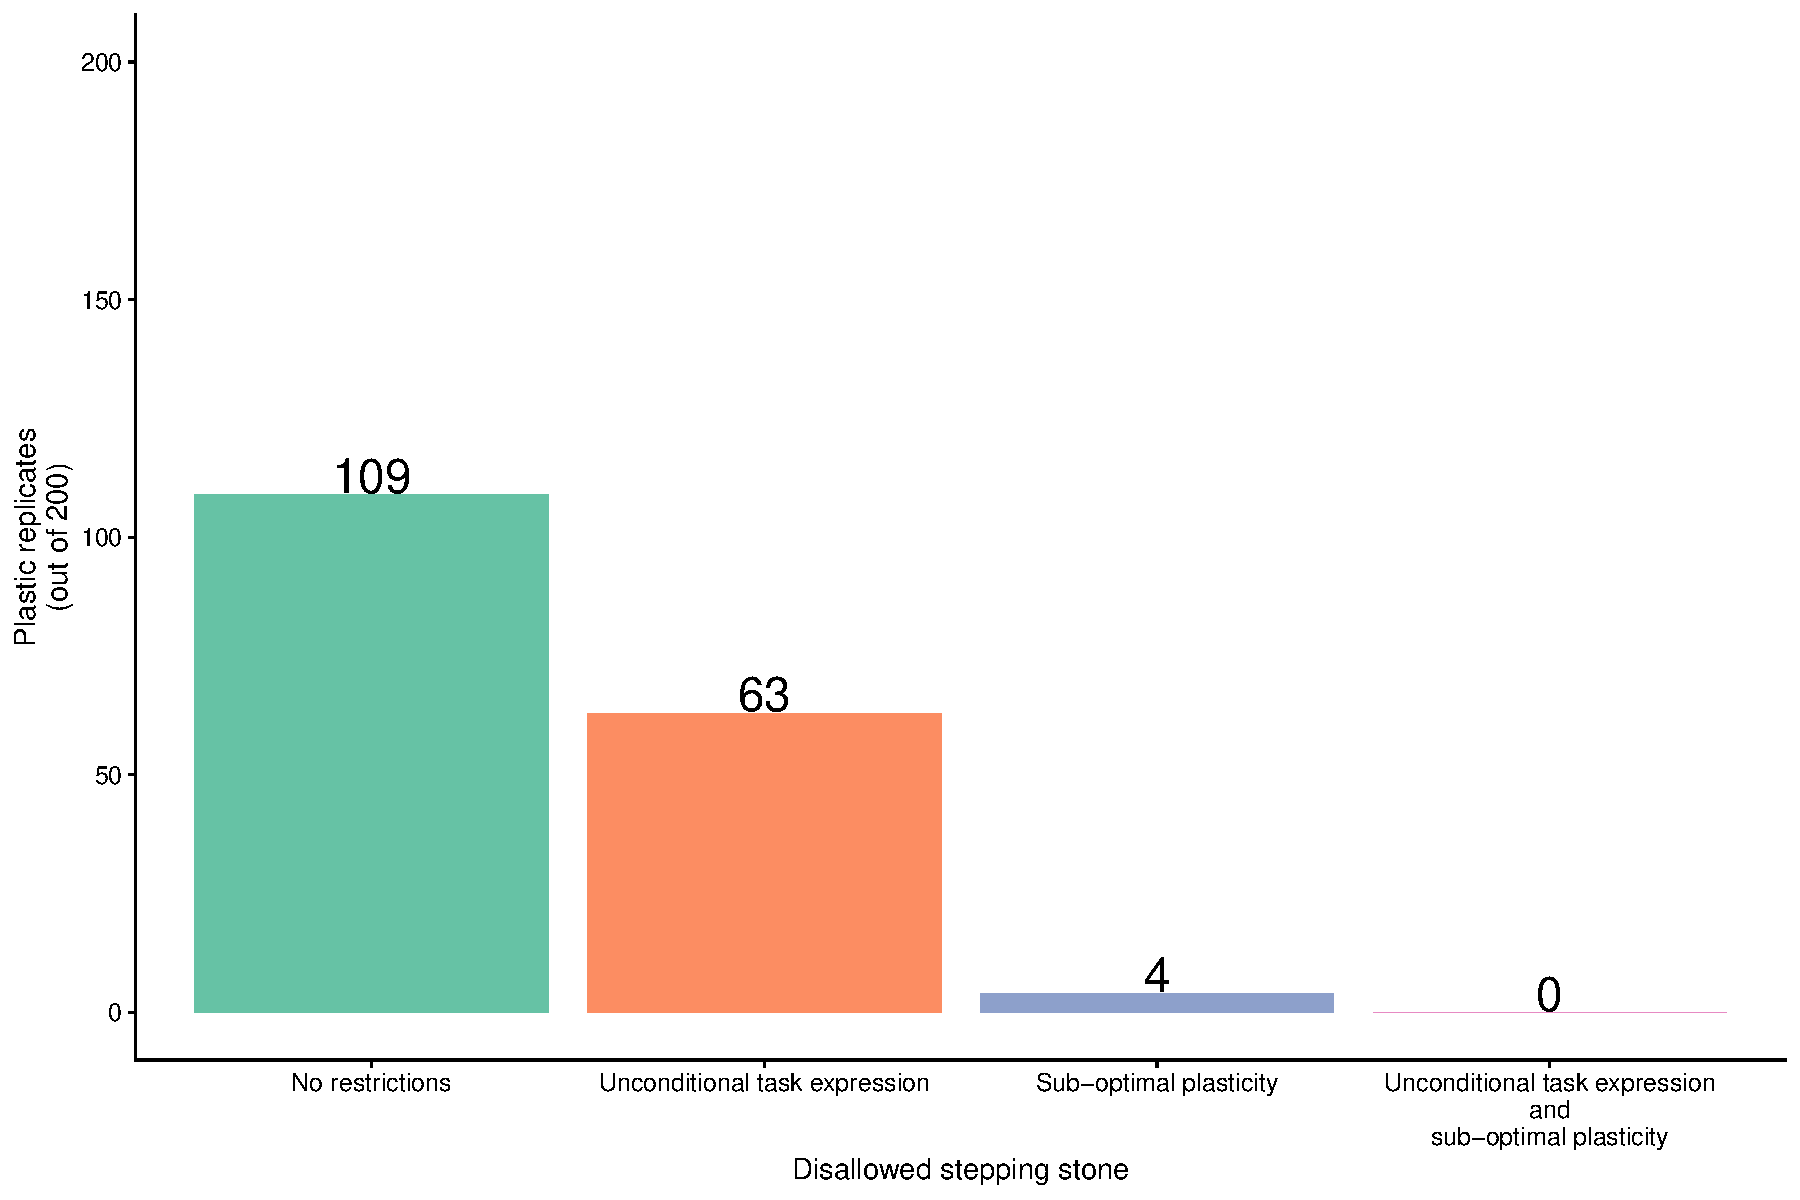
\includegraphics[height=0.3\textheight, keepaspectratio]
  {chapters/02-evolutionary-origins-of-plasticity/media/blocked-stepping-stones-baseline.pdf}
  \caption{\small A summary of evolutionary outcomes. 
  For each condition, the bar plot indicates the number of replicates (out of 200 per condition) where the final dominant genotype was plastic.
  }
  \label{chapter:origins-of-plasticity:fig:blocked-stepping-stones}
\end{figure*}

% Describe results
Figure \ref{chapter:origins-of-plasticity:fig:blocked-stepping-stones} gives the number of plastic replicates that evolved in each experimental condition.
We compared each of the three treatments that disallowed stepping stone phenotypes to our unmodified baseline treatment (Fisher's exact test with a significance level of 0.05 and a Bonferonni correction for multiple comparisons).
Each of the three treatments where we disallowed offspring with particular phenotypes had significantly fewer replicates with a plastic dominant genotype at the end of the experiment (unconditional trait expression disallowed: $p < 2e-05$; sub-optimal plasticity disallowed: $p<2e-16$; both unconditional trait expression and sub-optimal plasticity disallowed: $p<1e-16$).

% -- Discuss --
% No intermediate phenotypes => no plasticity evolves
No phenotypically plastic genotypes evolved when we disallowed all intermediate phenotypes (\textit{i.e.}, those that express NAND and/or NOT unconditionally and those that are sub-optimally plastic); when all intermediate phenotypes were disallowed, only two phenotypes were possible: (1) performing neither the NOT nor NAND tasks across environments (ENV-NAND and ENV-NOT) and (2) optimally regulating between the NOT and NAND tasks across environments.
For plasticity to evolve without allowing evolution to traverse intermediate stepping stones, optimal plasticity would need arise in a single mutational step from a genotype that performed neither the NAND nor NOT tasks.
This result demonstrates that, together, these intermediate phenotypes represent crucial building blocks for the evolution of phenotypic plasticity. 

% No unconditional task expression => less plasticity
% No sub-optimal plasticity => even less plasticity
When we prevented genotypes that perform tasks unconditionally across environments, plasticity evolved less frequently than in treatments where we placed no restrictions on phenotypes; this supports our previous observation that unconditional task expression is a stepping stone toward plastic task expression. However, many replicates (63 / 200) where unconditional task expression was disallowed still yielded plastic organisms. Thus, while unconditional trait expression is likely a valuable building block in the evolution of phenotypic plasticity, it is not necessary. Our results indicate that sub-optimal plasticity is a more important building block for optimal plasticity than unconditional trait expression. Only 4 / 200 replicates where we disallowed sub-optimally plastic phenotypes yielded optimal plasticity. This is not unsurprising, as a lineage would need to move from a state of unconditional task expression to perfect task regulation in a single mutational step.

\subsection{Are stochastic strategies evolving as an alternative to phenotypic plasticity?}

Stochastic phenotype switching---a form of bet hedging \citep{seger_what_1987}---is a common strategy leveraged by bacteria in fluctuating environments \citep{rainey_evolutionary_2011}. 
Unlike phenotypic plasticity where environmental conditions alter gene expression, stochastic phenotype switching relies on mutational input to induce phenotypic changes. 
This strategy is thought to be a viable alternative to phenotypic plasticity in the absence of reliable environmental signals or when the processing of sensory information is costly \citep{rainey_evolutionary_2011}.
Strategic stochastic phenotype switching often relies on contingency loci, which are hypermutable regions of the genome that can induce phenotype switching via mutational input \citep{moxon_bacterial_2006}. 

We hypothesized that stochastic phenotype switching was an alternative evolutionary strategy to phenotypic plasticity because of its commonality in bacteria. 
We most expected to see stochastic phenotype switching in our experimental treatments where the fewest number of replicates produced phenotypically plastic final, dominant genotypes. 

\subsubsection{Lineage Visualization}

It can be difficult to intuitively understand evolutionary strategies leveraged by a lineage without a visual aid.
To explore evolutionary strategies alternative to phenotypic plasticity in fluctuating environments, we visualized the lineages of dominant, non-plastic genotypes from our experimental treatments. 

\begin{figure*}[ht!]
  \centering
  \begin{minipage}[b]{\linewidth}
  \centering
  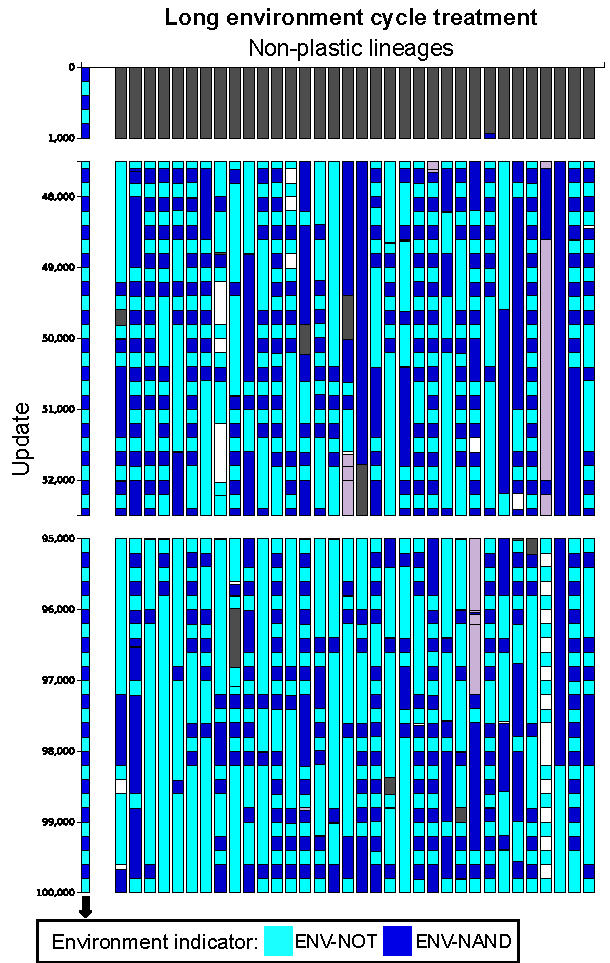
\includegraphics[height=0.4\textheight, keepaspectratio]
  {chapters/02-evolutionary-origins-of-plasticity/media/long-cycle-non-plastic-lineages.pdf}
  \caption{\small 
  Time-sliced lineage visualization of non-plastic, dominant genotypes from the long environment cycle treatment. 
  Abbreviated color reference: 
  cyan represents unconditional NOT task performance, 
  dark blue represents unconditional NAND task performance, 
  light purple represents sub-optimal forms of plasticity,
  and dark purple represents optimal plasticity. 
  Refer to Figure \ref{chapter:origins-of-plasticity:fig:task-profiles} for a full legend of phenotype colors.
  }
  \label{chapter:origins-of-plasticity:fig:long-cycle-lineages}
  \end{minipage}
\end{figure*}


If a lineage relied on stochastic phenotype switching, we would expect it to switch between phenotypic states of unconditional NAND task performance and unconditional NOT task performance in approximate synchronization with the changing environment. 
Specifically, we should see ancestors along a lineage perform NAND unconditionally during periods of ENV-NAND and see ancestors performing NOT unconditionally during periods of ENV-NOT. 
We show a time-sliced lineage visualization of dominant, non-plastic genotypes at the end of our experiment for the long-environment-cycle-length treatment (Figure \ref{chapter:origins-of-plasticity:fig:long-cycle-lineages}).  

From Figure \ref{chapter:origins-of-plasticity:fig:long-cycle-lineages}, we see what appear to be cases of stochastic phenotype switching.
That is, lineages switching between phenotypic states of unconditional NAND task performance and unconditional NOT task performance in approximate synchronization with the environment. 
Many of the lineages in the long-environment-cycle treatment seem to be undergoing stochastic phenotype switching. 
A few examples of what appear to be stochastic phenotype switching can even be seen in Figure \ref{chapter:origins-of-plasticity:fig:baseline-lineages} (the plastic lineages from our baseline treatment) between updates 47,500 and 52,500 (the middle time-slice), prompting the following open question: in addition to being an alternative strategy to plasticity in fluctuating environments, could stochastic phenotype switching also act as a precursor or building block toward plasticity? 

Our visualizations only provide an exploratory method for understanding evolutionary strategies employed by a lineage. 
Further analysis would be required to confirm or reject our hypothesis that stochastic phenotype switching is evolving as an alternative strategy to phenotypic plasticity in our system. 
This hypothesis is particularly worthwhile to explore because our mutation rate was fixed across the genome, preventing the evolution of contingency loci.  
Furthermore, because sensing mechanisms were perfectly accurate, phenotypic plasticity was a reliable strategy. 
We hypothesize that genotypes are moving to a region of the mutational landscape that straddles the boundary between expressing unconditional NAND task performance and unconditional NOT task performance such that minimal mutational input is required to switch phenotypes. 
This type of evolutionary trajectory has been demonstrated by Crombach and Hogeweg in evolutionary simulations of simple, genome-encoded gene regulatory network models \citep{crombach_evolution_2008}.
In their simulations, Crombach and Hogeweg found that networks evolved in an oscillating environment possessed genotype to phenotype mappings that were mutationally more efficient at generating adaptive phenotypes in alternative environments. 